%!TEX root = ../memoire.tex

\chapter{Génération automatique de texte}

%%%%%%%%%%%%%%%%%%%%%%%%%%%%%%%%%%%%%%%%%%%%%%%%%%%%%%%
% --------- I N T R O   ---------
%%%%%%%%%%%%%%%%%%%%%%%%%%%%%%%%%%%%%%%%%%%%%%%%%%%%%%%

La génération automatique de texte découle de la branche qu'est le \ac{TAL}. Reiter et Dale \citep{ReiterBuildingNaturalLanguage2000} définissent cette branche comme étant un domaine à la croisée des chemins entre l'intelligence artificielle et la linguistique computationnelle. L'objectif est de développer des sytèmes pouvant produire du texte compréhensible en langue naturelle à partir de données non-linguistiques. Bien que l'objectif est commun à tous ces systèmes, les moyens pour s'y rendre sont de divers ordres. Entre autre car il existe des inputs de diverses natures : données, texte et images \citep{thomason:coling14}. Ensuite car il y existe diverses approches de réalisation de texte : templates, règles, stochastiques \citep{gatt18}.

Toutefois, avant d'entrer dans les détails de la \ac{GAT}, il serait intéressant de mentionner l'origine de ces systèmes. À la base, ils ont été conçus pour, entre autre, générer des rapports automatiquement afin de faciliter le travail des humains. Effectivement, il est très utile pour certains de pouvoir lire un résumé de données numériques analysées par un système informatique. Tel que JSreal le mentionne, avec la GAT on peut présenter un résumé d'information provenant d'input numérique qui serait incompréhensible, mais utile pour un humain qui n'est pas un expert, et donc incapable de déchiffrer ces données. En plus d'être capable de résumé ces informations, le système informatique a l'avantage de fournir ces rapports sans se fatiguer à faire une tâche extrêmement monotone, qui pourrait être très coûteuse en termes de temps et de ressources pour des être humains.  D'ailleurs, pour qu'ils soient utiles, les textes générés automatiquement n'ont pas besoin d'être lus par une quantité phénomènale de gens. Dès qu'ils remplissent leur fonction, en étant utile à ne serait-ce que quelques personnes, leur raison d'être sera justifiée.  Dans cette même optique, il s'est développé des systèmes pouvant générer du texte en fonction de l'utilisateur. Ainsi, on pourrait générer un rapport X en fonction du professionnel, du technicien ou du client \citep{1948c0b7a8ca42679cad977bb2cdddc2} qui lira ce texte. Cette utilisation de la \ac{GAT} s'applique à de nombreux domaines dont les textes journalistiques. Les articles décrivant les matchs sportifs qui ne bénéficient pas de couverture médiatique \citep{W17-3513} sont des applications concrètes et utile du développement en \ac{GAT}. De même que des rapports générés automatiquement sur la qualité de l'air en fonction de l'utilisateur \citep{WannerMARQUISGENERATIONUSERTAILORED2010}.

De nos jours la \ac{GAT} a évolué depuis que Dale et Reiter ont publié leur livre. Bien que ce soit le livre le plus complet entourant la NLG, le domaine a changé avec l'émergence de text-to-text generation et de vision-to-text generation \citep{DBLP:journals/corr/HendricksARDSD16}. qui reposent plus sur des méthodes statistiques que les modèles traditionnels de data-to-text qui étaient rule-based ou template based \citep{gatt18}. D'ailleurs, les frontières entre les diverses approches s'affaissent aussi avec le temps et nous sommes témoins d'une apparition constante de systèmes hybrides. Par exemple, des systèmes à base de patrons utilisant des règles de grammaire, des systèmes à base de règles utilisant des méthodes statistiques pour combler certaines tâches \citep{gatt18}. C'est donc un domaine très vaste qui, à ce jour, n'est pas uniforme. Ce qui est directement lié à une grande variété en NLG: divers types d'input (type de données), divers objectifs (tâches), diverses approches. Il est aussi important de préciser que la \ac{GAT} a aussi une valeur linguistique théorique. Il existe des linguistes qui testent leur théories via le développement de générateur automatique de texte. C'est effectivement une bonne manière de vérifier si un modèle théorique fonctionne\citep{DanlosPresentationmodelegeneration1983}. 

Dans le cadre de ce mémoire, notre projet est un réalisateur. La réalisation linguistique étant une étape du processus entourant la \ac{GAT}, nous ne travaillons que sur celle-ci. D'ailleurs notre réalisateur est créé avec des perspectives linguistiques. Ce qui exclut les systèmes à base de patrons et les systèmes statistiques, car ceux-ci ne nécessitent pas d'analyse linguistique pour le bon fonctionnement de la réalisation. Notre système se base sur des règles grammaticales. Cependant, avant de décrire notre projet, nous allons jeter les bases de la \ac{GAT} en décrivant le pipeline classique et en exposant quelques réalisateurs linguistiques.

%%%%%%%%%%%%%%%%%%%%%%%%%%%%%%%%%%%%%%%%%%%%%%%%%%%%%%%
% --------- P I P E L I N E   ---------
%%%%%%%%%%%%%%%%%%%%%%%%%%%%%%%%%%%%%%%%%%%%%%%%%%%%%%%

\section{Pipeline classique GAT} \label{ppc}

À la base, le pipeline classique observé par Dale et Reiter est un processus séquentiel séparé en diverses sections \citep{ReiterBuildingNaturalLanguage2000}. Traditionnellement, les six étapes suivantes sont les plus utilisées selon Dale et Reiter, comme illustré à la figure~\ref{fig:Pipeline}.
%les figures latex bougent, donc évite les formulations comme ça.
\begin{figure}[htb] % utilise toujours [htb]
	\centering
	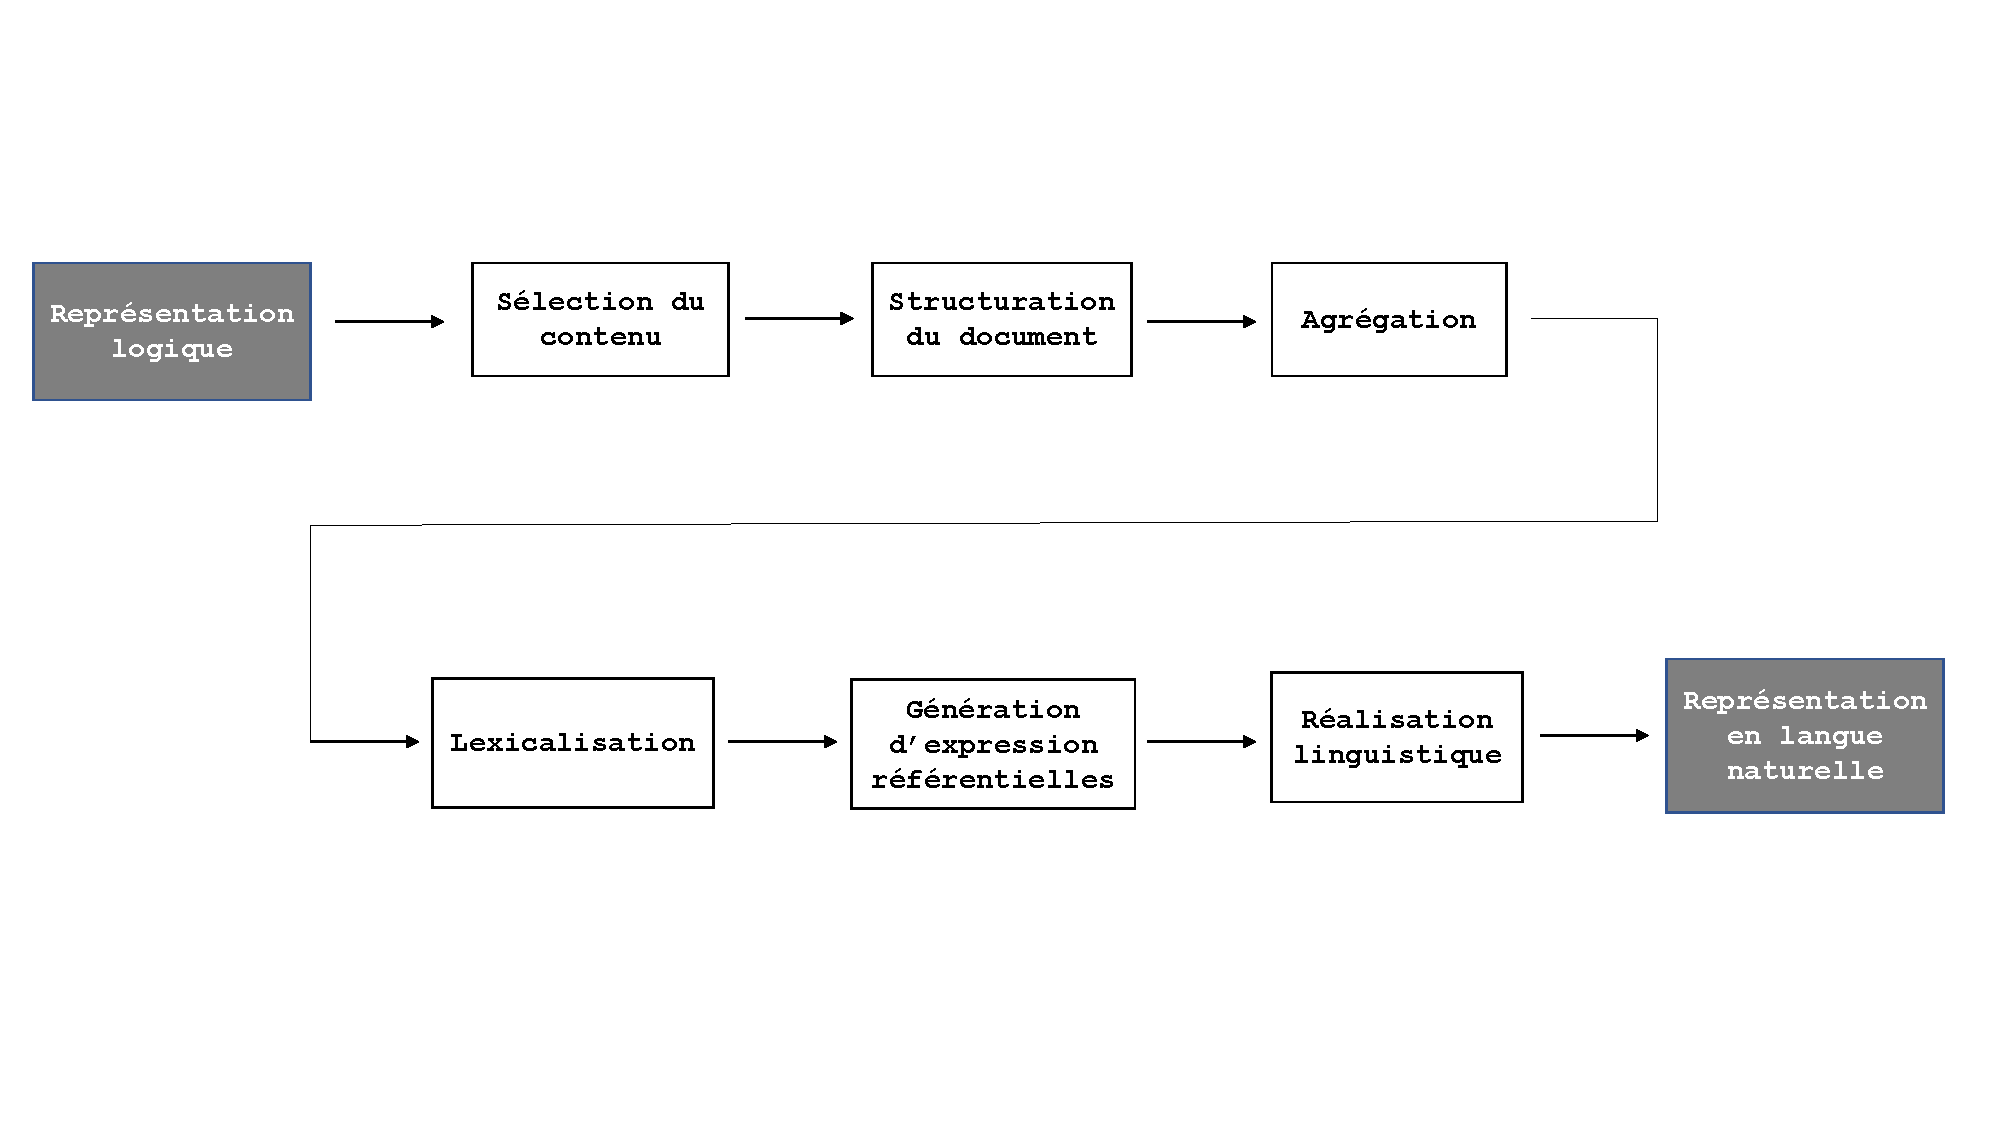
\includegraphics[width=1\textwidth, trim = {0cm 0cm 0cm 0cm},clip]{ch2/figs/pipeline.pdf}
	\caption{Pipeline classique}
	\label{fig:Pipeline}
\end{figure}

Beaucoup s'entendent pour dire qu'il y a deux parties. Le \emph{quoi-dire} et le \emph{comment-le-dire} selon \citep{DanlosPresentationmodelegeneration1983}, puis le \emph{early process} et le \emph{late process}  selon \citep{gatt18}. Le quoi-dire (\emph{early process}) fait référence à la sélection du contenu,la structuration de celle-ci et l'agrégation, puis le comment-le-dire (\emph{late process}) fait référence à toutes les étapes subséquentes : la lexicalisation, la génération d'expressions référentielles et la réalisation. Pour mieux comprendre le processus de \ac{GAT}, nous décrirons en quelques lignes chacune des étapes qui la compose.

\subsection{Sélection du contenu}

Un système de \ac{GAT} doit sélectionner quelles informations seront inclues dans le texte en construction et quelles informations n'y seront pas. La sélection du texte dépend entre autre de l'objectif de la tâche (par exemple si un texte est adressé à un débutant ou un expert), ainsi typiquement , il y a plus d'information ou de détails dans les données que d'information que nous voulons transmettre en texte. Ainsi, la sélection de contenu implique des choix. Par exemple, s'il s'agit de données pour un match de soccer, on ne voudrait probablement pas réaliser toutes les passes et les fautes commises durant le match, bien que ces informations figurent dans les données en input. Il faut donc les filtrer et créer des représentations sémantiques de l'information qui sont souvent exprimé en représentation formelle du langage comme des représentations logiques, des base de données, des matrices ou des graphes.

\subsection{Structuration du document}
Après avoir sélectionné le contenu, un système \ac{GAT} doit décider l'ordre dans lequel les informations seront présentées. Par exemple, si on utilise encore l'exemple du soccer, on commencerait par les informations générales liées au match (où et quand le match a eu lieu, entre quelles équipes, qui était blessé cette journée, etc), puis la description des buts comptés en ordre chronologique. Ce qui résulte de cette étape du processus est le plan d'un texte: une représentation ordonnée et structurée de messages à transmettre. Durant les dernières années, il y a eu des tentatives d'implémenter des méthodes d'apprentissage machine pour que la structuration de document se fasse automatiquement \citep{DimitromanolakiLearningOrderFacts2003}.

\subsection{Agrégation}
Ce ne sont pas tous les messages sélectionnés dans le plan qui doivent être exprimés dans des phrases individuelles. En combinant des phrases individuelles en une seule et même phrase, on génère un texte beaucoup plus fluide et agréable à lire \citep{ChengCapturingInteractionAggregation2000}. Ainsi, la majeure partie du temps, elle sert à enlever la redondance dans le texte. 

\subsection{Lexicalisation}
À cette étape, nous avons des données sélectionnées, puis structurées et que les futures phrases ont été combinées, on peut commencer à traduire les données en langue naturelle. Cette partie est très importante car c'est là qu'on choisi les mots qui seront utilisés pour transmettre le message. Toutefois, cette section se complique parfois car il existe naturellement plusieurs manières différentes de dire la même chose. La complexité de ce processus de lexicalisation dépend des mécanismes intégrés au système pour gérer cela. Certains traitent de lexicalisation en surface, d'autres la traite profondément. Toutefois, ceux qui traitent la lexicalisation en surface sont beaucoup plus restreints dans leur choix et sont très rigides. Tandis qu'un modèle profond permet de mieux tenir compte de la richesse lexicale d'une langue, mais il faudra une approche qui unit les représentations conceptuelles avec des règles de grammaire qui encoderont les choix lexicaux et syntaxiques. D'ailleurs, \citep{ElhadadFloatingConstraintsLexical1997} avait grandement contribué pour cela.

Convertir un graphe sémantique d'entités et de relations, en un graphe syntaxique de mots et de relations syntaxiques. 

\subsection{Génération d'expressions réferentielles}
Souvent référée comme étape discriminatoire dont le but est de déterminer quelles informations doivent être générées pour qu'on puisse distinguer toutes les entités en jeu. Le but est de s'assurer que le lecteur peut idientifier chaque entité dans le texte. La meilleure manière de référer à une entité donnée.
Il s'agit de la tâche pour sélectionner des mots ou des phrases qui identifieront des entités. C'est une étape du processus qui a reçu beaucoup d'attention, car il n'y a toujours pas de consensus quant à la manière de faire et c'est extrêmement difficle.

\subsection{Réalisation linguistique}
La dernière étape de ce pipeline NLG classique est la réalisation linguistique. Lorsque tous les mots, puis successivement les phrases ont été choisies, il faut les combiner en des phrases grammaticales. Cette tâche implique couramment l'application de traits morpho-syntaxiques et la linéarisation. De même qu'insérer les mots fonctionnels (auxiliaires, etc.) et la ponctuation. \citep{LambreyImplementationcollocationspour2017} Objectif: appliquer règles et procédés d'ordre grammaticaux aux représentations abstraites pour que l'output satisfasse les contraintes syntaxiques et morphologiques de la langue en question.

À ce sujet, il existe plusieurs approches effectuer la réalisation linguistique. D'abord, la réalisation à base de patrons, puis celle à base de règles et finalement, l'approche statistique.

\subsubsection{À base de patrons}
Cette approche est utilisée pour des systèmes de \ac{GAT} qui sont créés pour des domaines spécifiques (comme la météo ou les matchs sportifs) et dans lesquels les variations linguistiques sont restreintes à un minimum \citep{mcroy_channarukul_ali_2003}. Dans ces cas, les outputs peuvent être générés via des systèmes à base de patrons, comme le montre la phrase en \ref{template} provenant de \citep{gatt18}.
\ex. \label{template} \emph{Phrase générée à partir d'un réalisateur de type patrons}
	\a.\$player scored for \$team in the \$minute minute. 
	\b. Ivan Rakitic scored for Barcelona in the 4th minute.

En \ref{template}, on voit que ce patron contient trois variables (marquées par les \$) qui peuvent être comblées par un nom de joueur, suivi d'un nom d'équipe et d'une indication temporelle. Ce patron permet de générer une phrase en b). Cet exemple démontre bien l'avantage d'utiliser des réalisateurs à base de patrons. Ils permettent de prévoir ce qui sera généré en output, ce qui diminue les risques d'erreurs. D'ailleurs, ils peuvent être complémentés par des règles de grammaire, ce qui les rend très performants. Toutefois, puisqu'ils sont codés à la main, ces sytèmes ont l'inconvénient d'être long à construire et coûteux en termes de temps. On notera toutefois que ces systèmes peuvent aussi être combinés à de l'apprentissage machine. Les rendant capable d'apprendre à écrire des patrons.

\subsubsection{À base de règles grammaticales}
Les modèles à base de règles grammaticales s'emploient autant des les domaines spécifiques que les domaines généraux. Effectivement, ils se prêtent bien à la réalisation de domaine général car ils ont comme fonction de pouvoir réaliser du texte de la manière la plus humaine et naturelle possible puisqu'ils se basent sur des théories linguistiques qui modélisent déjà le langage. Tous les choix à faire dans la tâche de réalisation sont laissés aux soin de la grammaire qui effectuera les règles nécessaires à la bonne formation de phrases. Les grammaires sont écrites à la main et sont généralement inspirées de cadres théoriques déjà éxistantes. Les choix qui mèneront à la génération de texte dépendent des unités lexicales et des règles de grammaires combinées. Ce qui nécessite que les systèmes sont codés très minutieusement, puisque les langues naturelles sont complexes et très riches.

\subsubsection{Statistiques}

Avec des modules d'apprentissage machine, on peut acquérir des grammaires probabilistes \citep{gatt18}. Ce qui permet à la fois d'agrandir la couverture des réalisateurs et de diminuer la charge de travail manuelle. On entraîne ces systèmes à générer du texte à partir de méthodes statistiques, ce qui ne requiert pas d'écrire manuellement des grammaires.

\subsubsection{Règles versus statistiques}

Tel que Belz le dit, traditionnellement, les systèmes de \ac{GAT} tendaient vers des ressources crées manuellement (dictionnaires et grammaires). De tels systèmes sont longs à créer et difficile à plugger à des pipelines.Dans les dernières décennies, plusieurs chercheurs ont voulu automatisés l'acquisition de grammaires et dictionnaires via du machine learning \citep{LangkildeForestbasedStatisticalSentence2000}. Tel que Belz le dit, des systèmes qui incorporent la composante d'entraînement semblent plus facile à plugger dans des pipelines. Toutefois, les méthodes automatiques sont souvent vues comme une amélioration irréfutables aux systèmes de \ac{GAT}. Belz s'est posée la question à savoir si effectivement c'était irréfutablement une bonne chose que les systèmes s'automatisent de plus en plus\citep{BelzSystemBuildingCost2009}. Elle se demandait si la diminution du temps à implémenter des systèmes et leur plus grande adaptabilité se fait au détriment de la qualité de l'output, et si c'est le cas, jusqu'à quel point la qualité de l'output est affectée. La conclusion est que les systèmes créé manuellement sont généralement préféré des humains lors des human evaluations, et que les metrics system pour évaluer les réalisateurs automatiques surévalue parfois les systèmes statistiques et sous-évalue les systèmes manuels\citep{BelzSystemBuildingCost2009}.

Dans son blog, E.Reiter \citep{ReiterNaturalLanguageGeneration2016} nous fait part de ses réflexions par rapport au \emph{machine learning}. Même si les ML systèmes en \ac{GAT} génèrent du bon texte la plupart du temps, ils peuvent occasionnellement générer du texte bizarre et inapproprié (et les évaluations sont souvent basés sur la moyenne du bon texte généré et pas par rapport aux incongruités générées). Et lorsque ça arrive, les systèmes basés sur des méthodes statistiques sont difficile à corriger car le tout est basé sur les statistiques, contrairement aux rule-based où on peut cerner le problème avec plus de facilité et le corriger.) Ce comportement est acceptalbe dans certains contextes (comme la description d'images), mais pas approprié pour des systèmes de \ac{GAT} qui génèrent du texte destiné à des gens qui prendront ensuite des décisions basées sur ces textes. Par contre, il termine son blog en soulignant que la \ac{GAT} a aussi beaucoup à gagner des méthodes statistiques, mais plutôt comme outils que comme base.

Pour ces raisons, nous avons décidé de travailler sur un réalisateur à base de règles. D'ailleurs, la section suivante présentera des réalisateurs utilisés dans des tâches en \ac{GAT}

\draft{Les réalisateurs profonds ont aussi de la difficulté (choix lexical est rigide) à traiter les collocations \citep{lareau18}}

%%%%%%%%%%%%%%%%%%%%%%%%%%%%%%%%%%%%%%%%%%%%%%%%%%%%%%%
% --------- R É A L I S A T I O N   ---------
%%%%%%%%%%%%%%%%%%%%%%%%%%%%%%%%%%%%%%%%%%%%%%%%%%%%%%%


\section{Réalisation}

Notre projet consiste à doter un réalisateur profond d'un dictionnaire verbal riche pour lui permettre de couvrir toute la grammaire anglaise. Donc, pour une meilleure compréhension de la tâche qu'est la réalisation de texte, nous décrirons quelques réalisateurs brièvement.

Tel qu'explicité à la figure~\ref{fig:Pipeline}, la réalisation est la dernière étape dans le processus de \ac{GAT}. Toutefois, pour beaucoup de chercheurs, elle ne représente pas uniquement les tâches décrites précédemment. Il règne une ambiguité quant aux concepts qu'incarne la réalisation. Lambrey le mentionne \citep{LambreyImplementationcollocationspour2017} dans son mémoire, effectivement, le terme technique \emph{réalisation} peut faire référence, à la fois aux systèmes qui performent la tâche de réalisation linguistique telle que décrite dans le pipeline classique (référer au point), mais elle réfère aussi aux engins qui opèrent la réalisation ainsi que des tâches se trouvant en amont de la réalisation classique (notamment la lexicalisation). Nous utiliserons dans ce mémoire les mêmes disctinctions que \citep{LambreyImplementationcollocationspour2017}. Ainsi, on appellera un réalisateur de surface un engin qui s'occupe de la réalisation linguistique à un niveau plus superficiel, prenant comme input des structures syntaxiques dont les unités sont déjà lexicalisées. On appellera un réalisateur profond un système qui effectue la réalisation en partant d'un niveau plus abstrait, c'est-à-dire généralement un niveau sémantique et dont les unités ne sont pas lexicalisées dans l'input. Ces réalisateurs profonds nécessitent des dictionnaires explicitant la combinatoire des unités lexicales et des grammaires plus complexes afin de traiter l'interface sémantique-syntaxe. Ces systèmes sont généralement liés à une théorie linguistique permettant de modéliser l'interaction entre l'input, le dictionnaire, la grammaire et l'output.

Puisqu'un système de \ac{GAT} complet est très coûteux en termes de temps et de ressource, il n'est pas rare que les chercheurs empruntent des réalisateurs déjà existant sur le marché \citep{EssersChoosingSurfaceRealiser1998}. Ainsi, dans les prochaines sections, nous décrirons certains réalisateurs de surface ou profonds.


%%%%%%%%%%%%%%%%%%%%%%%%%%%%%%%%%%%%%%%%%%%%%%%%%%%%%%%
% --------- R É A L I S A T E U R   S U R F A C E ---
%%%%%%%%%%%%%%%%%%%%%%%%%%%%%%%%%%%%%%%%%%%%%%%%%%%%%%%

\subsection{Réalisateurs de surface}

Parmi les premiers réalisateurs à base de règles, les choix qui mèneront à la génération de texte dépendent des unités lexicales et des règles de grammaires combinées. Ce qui nécessite que les systèmes sont codés très minutieusement, puisque les langues naturelles sont complexes et très riches. Ces systèmes exigent des niveaux de détails qui demande beaucoup de temps à créer et les rendant plus difficile à insérer dans le pipeline classique. C'est ce qui les distingue des réalisateurs profonds c'est qu'ils ne requièrent pas de théorie linguistique sous-jacente en raison de leur traitement du langage en surface. Les réalisateurs de surface sont généralement plus simples à utiliser et à implémanter dans un pipeline de \ac{GAT} \citep{gatt18} en raison de \draft{en raison de quoi? Parce que les choix lexicaux et les structures syntaxiques ont déjà été effectué \citep{lareau18}}. Les choix lexicaux étant déjà fait avant l'étape de réalisation, les réalisateurs de surface prennent en input une représentation syntaxique, donc lexicalisée. Dans ces systèmes, les dictionnaires et règles traitent l'interface morpho-syntaxique. Finalement, ils correspondent plus à la phase de réalisation mentionnée dans le pipeline classique de Dale et Reiter.

\subsubsection{SimpleNLG}
SimpleNLG est \citep{GattSimpleNLGRealisationEngine2009} est un réalisateur de surface écrit en java. Il opère une réalisation de surface à partir d'une structure syntaxique déjà lexicalisée encodée en XML. Par la suite, SimpleNLG opère les opérations morphologiques nécessaires (flexion, dérivation des mots, linéarisation, ajout d'auxiliaires, gestion de l'accord) puis linéarise le texte en sortie.

Le réalisateur est doté d'une grammaire et d'un dictionnaire. Ce dernier encode les propriétés syntaxiques et morphologiques. Le module grammaticale contient aussi de l'information de nature morpho-syntaxiques, il est composé de règles permettant de passer de l'interace syntaxique à l'interface morphologique.

SimpleNLG découpe son processus de réalisation en quatre étpaes. Premièrement, les lexèmes compris dans la structure d'input sont matchés avec l'entrée lexicale qui leur corresponde. Deuxièmement, il faut déterminer les traits lexicaux attachés à ces entrées. Puis, troisièmement, les lexèmes sont combinés entre eux pour former des syntagmes de plus en plus grand jusqu'à ce que l'entièreté de la phrase forme un syntagme. Finalement, ces syntagmes sont linéarisés puis les règles morphologiques s'appliquent pour obtenir les formes fléchies et éventuellement la phrase désirée en output.

Noter que SimpleNLG a été traduit dans plusieurs langues : espagnol, italien, et français, portugais (Mazzei et al., 2016, Ramos-Soto 2017, Vaudry et Lapalme 2013 ; Oliveira et Sripada)

\begin{lstlisting}[language=Xml, caption=Structure d'input dans SimpleNLG, label=simplenlg]
<Document>
  <child xsi:type="SPhraseSpec">
    <subj xsi:type="VPPhraseSpec" FORM="PRESENT_PARTICIPLE">
      <head cat="VERB">
        <base>refactor</base>
      </head>
    </subj>
    <vp xsi:type="VPPhraseSpec" TENSE="PRESENT" >
      <head cat="VERB">
        <base>be</base>
      </head>
      <compl xsi:type="VPPhraseSpec" FORM="PAST_PARTICIPLE">
        <head cat="VERB">
          <base>need</base>
        </head>
      </compl>
    </vp>
  </child>
</Document>
\end{lstlisting}
La figure \ref{simplenlg} permet de réaliser la phrase 'Refactoring is needed.'

\subsubsection{JSreal}
JSreal \citep{DaoustJSREALTextRealizer2015} qui est en fait JavaScript Realiser. C'est un réaliseur de texte orienté pour les programmeurs web. C'est un réaliseur de texte en français qui génère des expressions et phrases bien formées qui elles peuvent être formattées en HTML pour être exposé dans un fureteur. Il peut aussi s'employer seul à des fins purement linguistiques ou être intégéré dans des générateurs de textes. Les Specs de JSreal sont similaires à ceux de SimpleNLG.

Pour générer du texte JSreal prend en input des structures syntaxiques lexicalisées. La bonne construction de la phrase provient du fait que les constituants de les structures syntaxiques vont faire appel à des règles, qui elles opèrent la combinaison des syntagmes entre eux jusqu'à ce que la structure au complet ait été parsée. Pour générer du texte, JSreal possède les modules suivants : un dictionnaire et une grammaire (règles syntaxiques et morphologiques). Son dictionnaire défini la catégorie des mots qui le peuple, et les traits lexicaux attachés (genre, nombre, irrégularités, etc.). Les règles morpho-syntaxiques permettent de : .Il existe aussi une version bilingue de JSreal \citep{MolinsJSrealBBilingualText2015}.

\begin{lstlisting}[language=Xml, caption=JSreal, label=jsreal]
JSrealLoader({
        language: "en",
        lexiconUrl: URL.lexicon.en,
        ruleUrl: URL.rule.en,
        featureUrl: URL.feature
    }, function() {
    QUnit.test( "Sentence EN", function( assert ) {
        assert.equal(
            S(
                NP(D("the"), N("cat")),
                VP(V("sit"), PP(P("on"), NP(D("the"), N("coach")))).t("ps")
            )
        
\end{lstlisting}
La figure \ref{jsreal} produit la phrase :'The cat sat on the coach.'
		
\subsubsection{RealPro}
RealPro est implémenté en C++ \citep{LavoieFastPortableRealizer1997}. Il prend en input des arbres de dépendances.Le plus profond des réalisateurs de surface présénté jusqu'ici. La linéarisation s'opère entre le passage de la structure syntaxique de surface à la structure morphologique profonde. L'architecture de RealPro est basé sur la TST (citation). Brièvement, il s'agit d'une théorie qui schématise le langage en divers niveaux de représentations partant de la sémantique, syntaxe, morpho,phono, phoné. Ainsi, pour passer de la structure profonde à la strucutre de surface, le logiciel vérifie dans son dictionnaire (catégorie et information morphologique)et ses règles de grammaires pour s'assurer que le passage est grammatical. Ses connaissances lexicales sont encodées dans 2 modules: un dictionnaire et des règles de grammaires. Ceux-ci seront réquisitionnés par les diverses composantes au cours de la réalisation. Voici un graphique qui démontre leurs intéractions lors de la réalisation.
\begin{figure}[htb]
	\centering
	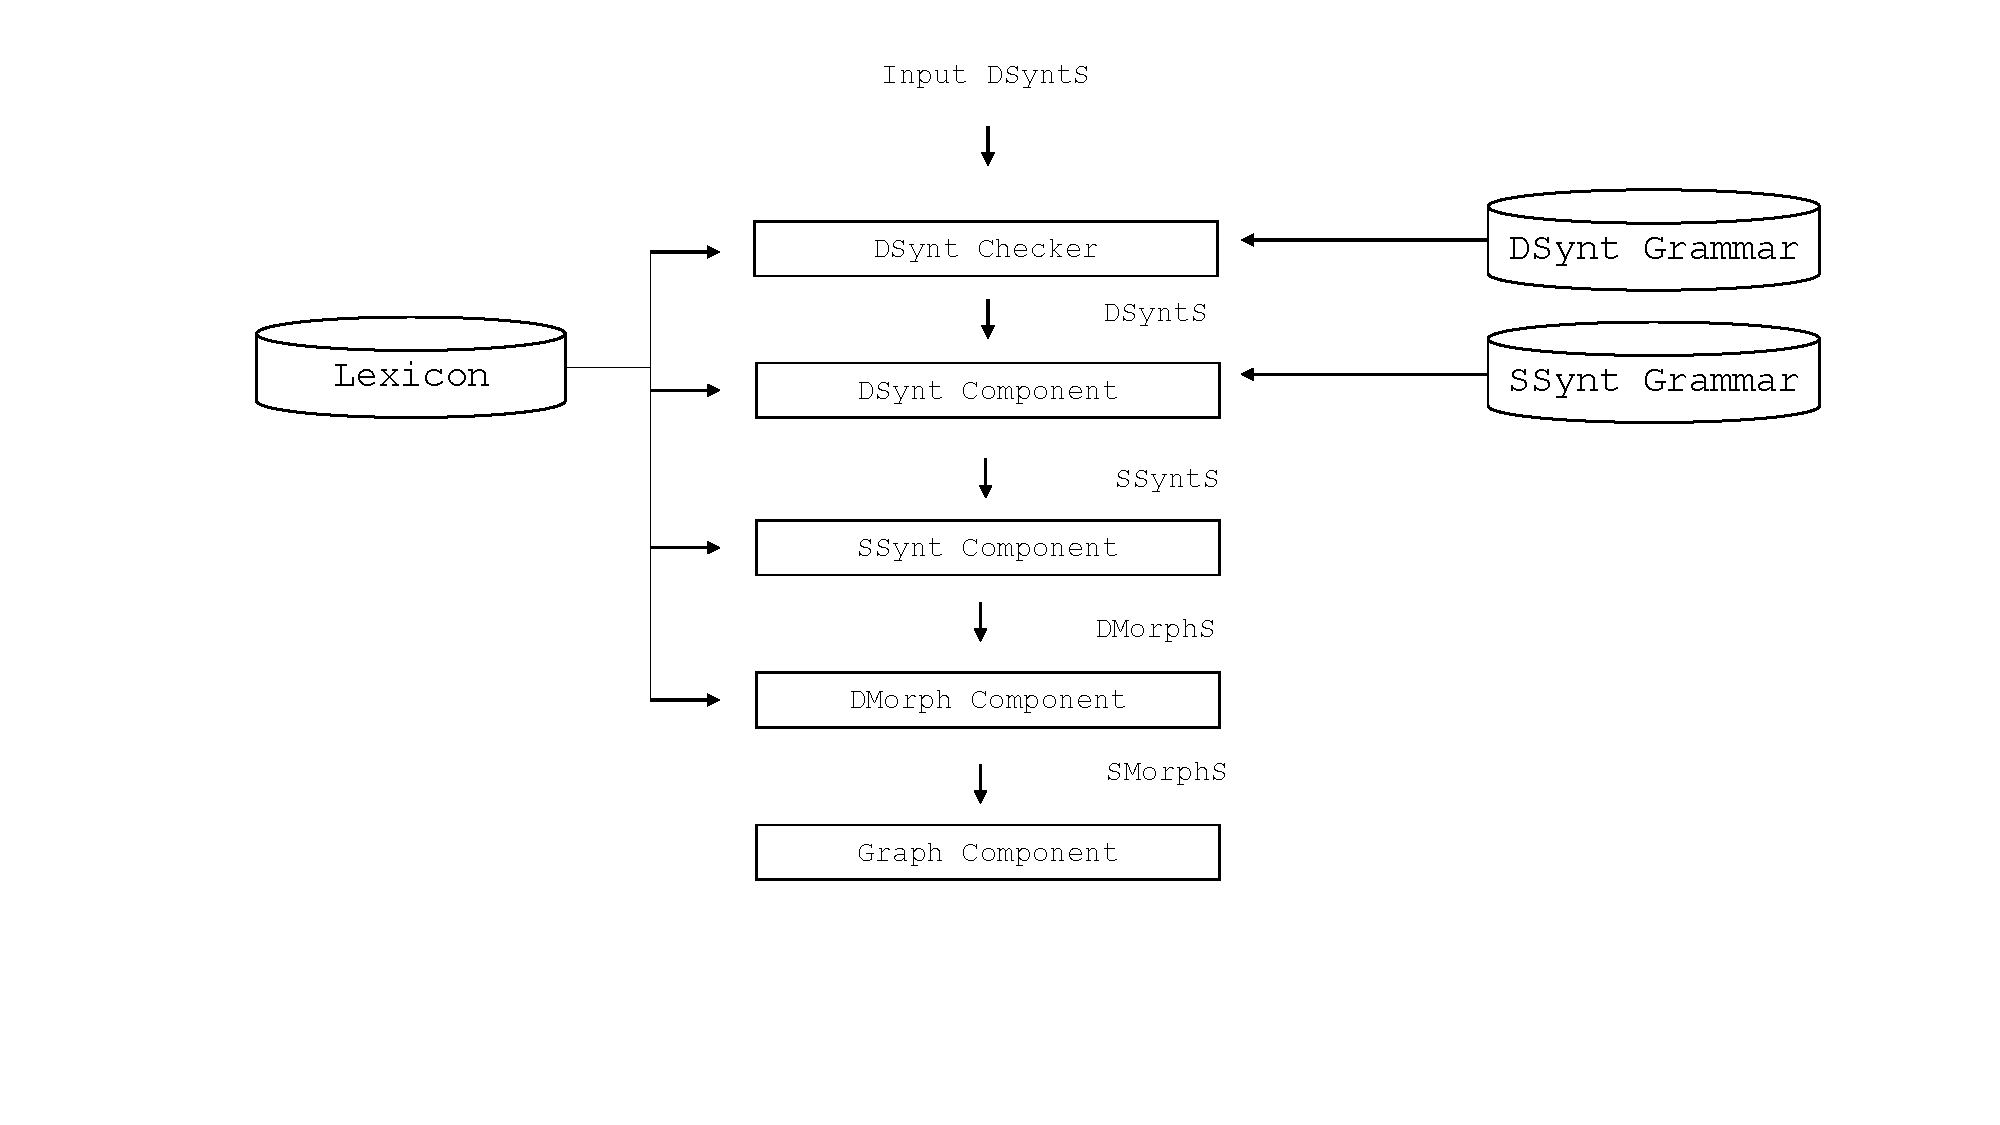
\includegraphics[width=1\textwidth, trim = {0cm 0cm 0cm 0cm},clip]{ch2/figs/realpro.pdf}
	\caption{RealPro}
	\label{fig:RealPro}
\end{figure}

\begin{lstlisting}[language=Xml, caption=Input, label=realpro]
HAVE1 [tense:past]
(I March [class:proper-noun]
II day [class:common-noun numberpl]
(ATTR rainy [class:adjective]))
\end{lstlisting}

Structure \ref{realpro} de dépendance représentant la phrase 'March had some rain days.'
%%%%%%%%%%%%%%%%%%%%%%%%%%%%%%%%%%%%%%%%%%%%%%%%%%%%%%%
% --------- R É A L I S A T E U R    P R O F O N D  ---
%%%%%%%%%%%%%%%%%%%%%%%%%%%%%%%%%%%%%%%%%%%%%%%%%%%%%%%

\subsection{Réalisateurs profonds}

\draft{
Maintenant que nous avons exposé quelques générateurs de surface, nous exposerons des réalisateurs profonds. Généralement, ceux-ci sont construits autour d'une théorie linguistique sous-jacente afin de rendre compte des multiples phénomènes linguistiques plus profonds que permet l'interface morpho-syntaxique. Effectivement, on peut plus facilement construire un système profond en se basant sur un modèle théorique. Ces modèles permettent de prendre un input plus abstrait que les structures syntaxiques.

En prenant comme input des réseaux sémantiques on permet une plus grande flexibilité dans le contenu généré. Lorsque le choix lexical n'est pas encore fait au moment de la réalisation, il est encore possible de générer une même idée en différentes constructions. Dans le pipeline classique, la lexicalisation est opérée avant la réalisation, faisant en sorte que les inputs contiennent des lexèmes déjà choisis. Cela restreint le nombre de constructions possibles. Finalement, tel que Polguère le dit \citep{PolguerePourmodelestratifie}, si on veut un système qui génère du texte de la manière la plus naturelle possible, il faut qu'un réalisateur linguistique incorporte la lexicalisation. Ainsi, on prend en input des structures conceptuelles qui véhiculent des idées et non des lexèmes. En prenant des inputs qui véhiculent des concepts(idées), le choix du lexème aura un impact direct sur la réalisation finale de l'énoncé. Cela nous permet de réaliser le langage dans toute sa complexité car des structures déjà lexicalisées sont très rigides et moins flexibles.}

\subsubsection{KPML}
KMPL\citep{BatemanEnablingTechnologyMultilingual1997} est un réalisateur linguistique multilingue issu du système PENMAN \citep{PenmanOverview}. C'est un système basé sur la grammaire fonctionnelle systémique (SFG) \citep{MatthiessenSystemicfunctionalgrammar1997}. Dans cette théorie, \draft{chaque choix linguistique est motivé par l'accomplissement d'une fonction. Cette perspective fonctionnaliste alimente l'aspect multilingue de KPML : les différentes langues partagent un certain nombre de fonctions. Seule la réalisation linguistique des fonctions diffère d'une langue à l'autre }.

\draft{La grammaire de KPML est encodée comme un réseau de système orienté (lisible de gauche à droite). Chaque intersection représente un choix grammatical minimal entre différents traits fonctionnels. Plus on avance dans le graphe, plus les choix deviennent spécifiques et précis. Cette architecture en réseau couvre tous les aspects linguistiques (phonologie, morphologie, syntaxe, etc.).}

Les structures d'input de ce système peuvent être de divers ordres: sémantiques et syntaxiques. Courte explication de la SFG : ressemble à la TST. Dans ce formalisme, la forme de surface est la conséquence directe de la sélection d'un ensemble de traits fonctionnels abstraits à partir d'une description des ressources du langage. Ces ressources sont représentées par des réseaux systémiques et dans ce formalisme la réalisation linguistique se fait en traversant les réseaux.

KPML prend des SPL en entrée. Il s'agit d'un acronyme pour \emph{Sentence Planning Language}. Un SPL est une matrice dont les objets sont des attributs et leurs valeurs.
\draft{Il traverse ses réseaux et produit un ensemble de déclarations de réalisation qui caractérisent le texte à générer, ces déclarations s'instanciant par des contraintes sur la forme grammaticale de la phrase. Ces contraintes sont spécifiées sous forme de matrices de traits grammaticaux. KPML arrive donc à généraliser beaucoup de phénomènes linguistiques grâce à ces réseaux.}

Afin d'illustrer à quoi ressemble l'input, nous allons reprendre un exemple de Dalet et Reiter: 'March had some rainy days'.
\begin{lstlisting}[language=Xml, caption=SPL: input de KPML, label=kpml]
(S1 \ generalized-possession
  :tense past 
	:domain (N1 \ time-interval
	            :lex march
							:determiner zero)
	:range (N2 \ time-interval
	           :number plural
						 :lex day
						 :determiner some
						 :property ascription
						 (A1 \ quality :lex rainy)))
\end{lstlisting}

\subsubsection{Surge}
\citep{Elhadad98surge:a}
Surge, qui signifie \emph{Systemic Unification Realisation Grammar of English}, est une grammaire de l'anglais. Elle est écrite en FUF\emph{Functional Unification Formalism} qui est basé sur FUG \citep{KayFunctionalUnificationGrammar1984}. FUF est un langage de programmation créé pour construire des grammaires computationnelles, plus particulièrement pour les besoins de la réalisation linguistique dans un cadre de grammaire d'unification. \draft{Son fonctionnement se base sur l'unification de graphes pour combiner une structure d'entrée (spécification de phrase) avec une grammaire de la langue de sortie. Le résultat est une structure spécifiée syntaxiquement qui est par la suite linéarisée pour produire la phrase finale.}

\draft{FUF prend en entrée des descriptions fonctionnelles (FD) décrivant le sens d'une phrase et une grammaire (aussi décrites en descriptions fonctionnelles). Ces descriptions fonctionnelles apparaissent sous la forme de matrices attributs-valeurs enchâssées. Le format de sortie est une phrase en anglais exprimant le sens voulu et suivant les normes grammaticales décrites par la grammaire}

Ils se servent de graphes d'unification comme input à leur système. Cet input est sous forme de FD (Functional Description), il s'agit d'une collection de paires attributs-valeurs dont l'union fournit une spécification de l'énoncé à génerer.

Nous reprendrons encore un exemple tiré de Dale et Reiter: 'March had some rainy days'.
\begin{lstlisting}[language=Xml, caption=FD: input de Surge, label=surge]
((cat clause)
 (proc ((type possessive)))
 (tense past)
 (partic ((possessor ((cat proper) head ((lex "March"))))
					(possessed ((cat common) head ((lex day)))
											(describer ((lex rainy)))
											(selective yes) (number plural)))))
\end{lstlisting}

Contrairement aux autres réalisateurs présentés ici, FUF n'utilise pas de dictionnaires, l'information lexicale est encodée dans la structure d'input.\draft{Le processus de réalisation profonde s'effectue en deux étapes. La première consiste à unifier les descriptions fonctionnelles du sens de la phrase à générer, c’est-à-dire enrichir la structure d’entrée, avec les spécifications syntaxiques et morphosyntaxiques de la grammaire. Ces spécifications permettent de gérer l'ordonnancement des mots, les constructions syntaxiques, l'accord, etc. Une fois l'unification terminée et la structure d'entrée enrichie, FUF linéarise la structure pour obtenir une phrase et prend en charge les contraintes morphologiques.}

\subsubsection{Forge}
FORGe est un transducteur de graphes qui génère du texte à l'aide de ressources lexicales dictionnairiques et grammaticales \citep{MilledemoFORGePompeu2017}. C'est un réalisateur profond qui hérite de l'architecture de MARQUIS \citep{WannerMARQUISGENERATIONUSERTAILORED2010}.  Il prend en entrée des représentations abstraites. Le système a été conçu pour l'anglais à la base, mais il se veut multilingue (espagnol, allemand, français et polonais sont en développement). C'est un système qui se base sur la théorie sens-texte \citep{melcuk1988}.

Input: représentations sémantiques composées de relations prédicats-arguments \draft{Voir la figure de MARQUIS : fonctionne de la même manière}

Génération de structures syntaxiques profonds: Dans ce système, la structure syntaxique et la lexicalisation se font en même temps pour s'assurer que la structure résultante est conforme aux règles grammaticales et aux contraintes lexicales. Ainsi, les noeuds syntaxiques sont étiquettés par une partie de discours, et lors du passage de la sémantique à la syntaxe, on vérifie que le lexème qui consommera le noeud correspond à la partie du discours requise par ce noeud. De cette manière, l'arbre est construit via un parsing successif du haut vers le bas. Ainsi, le noeud est lexicalisé et la structure des dépendants syntaxiques est créé en même temps, puis on vérifie que la partie du discours attribuée aux noeuds des dépendants correspond au lexème choisi par le système pour que ce soit une arbre de bonne forme. L'opération est effectuée successivement jusqu'à ce que toute la représentation sémantique ait été analysée. Il s'agit là du passage de la sémantique à la syntaxe, et il se fait via la combinaison des règles de l'interface en question et du dictionnaire.

Passage de la représentation sémantique à la structure syntaxique profonde via un parsing récursif top-down. Le top étant la racine syntaxique de la structure en développement, et une fois que le top est lexicalisé en syntaxe, on crée la structure qui lie ses dépendants syntaxiques, et les dépendants syntaxiques de ceux-ci jusqu'à ce qu'on parse la représentation sémantique au complet. \draft{Utiliser l'exemple fournit par eux, le refaire dans powerpoint}

Ensuite, le passage de la syntaxe profonde à la syntaxe de surface où on introduit les mots fonctionnels (prépositions, auxiliaires, déterminants). Cette étape est possible grâce à la complexité des dictionnaires qu'ils utilisent. Par exemple, pour réaliser la bonne préposition en surface, ils ont implémenté un dictionnaire de valence à leur système.

Finalement, la dernière étape consiste à appliquer les règles morpho-syntaxiques aux lexèmes, puis le tout est linéariser.

pipeline multilingue et flexible: S'adaptent à différents type d'input assez facilement. Premièrement, la preuve a été fournie lors de la compétition SemEval 2017 où ils ont adapté leur format d'input à celui requis par la compétiton, ça ne leur a pris qu'une semaine \citep{DBLP:conf/semeval/MilleCBW17}. C'est un réalisateur qui peut aisément générer du texte en différentes langues grâce à ses règles grammaticales qui sont majoritairement language-independent. Les autres règles qui sont propres à l'anglais peuvent aisément être adaptées à d'autres langues. En conclusion, avec des ressources lexicales riches, on peut générer du texte dans plusieurs langues en peu d'efforts. D'ailleurs, les auteurs mentionnent que certains modules du systèmes peuvent être complémentés avec des méthodes statisitques, ce qui lui donne la possibilité de couvrir plus large.

\subsubsection{MARQUIS}
Contrairemnt aux autres systèmes présentés ici, MARQUIS n'est pas qu'un réalisateur profond. Il s'agit d'un système de \ac{GAT} qui effectue toutes les étapes du processus de génération automatique de texte (section \ref{ppc}). Cependant, nous ne nous intéresserons qu'à l'aspect réalisation profonde de MARQUIS, pour plus d'informations, nous vous réferons à l'article \citep{WannerMARQUISGENERATIONUSERTAILORED2010}. 

MARQUIS est ainsi un projet dont le but est de générer à partir de données des bulletins météorologiques multilingue sur la qualité de l'air. Ces bulletins sont générés en fonction de l'utilisateur. Ainsi, la personne qui fait la requête d'un tel rapport entre ses informations personnelles et le bulletin sera générée en fonction de son expertise et de ses conditions médicales. Ainsi, un non-expert asthmatique se verra offrir un bulletin en fonction pouvant être lu par un non-expert et les données seront orientées en fonction de sa condition physique. Dans le cadre de ce travail, la partie qui décide le quoi-dire ne sera pas décrite ici. On décrira plutôt comment le système procède à la réalisation du message sélectionné par l'utilisateur.

\draft{question pour françois : pourquoi c'est uniquement la structure conceptuelle qui est partagée entre les langues et que la structure sémantique est language-dependent}

MARQUIS est aussi un système basé sur la Théorie Sens-Texte.
\draft{Le module de génération de surface de MARQUIS s'articule autour de six niveaux : conceptuel, sémantique, syntaxique profond, syntaxique de surface, morphologique (profond et de surface) et textuel. Pour passer d’un niveau à l'autre, MARQUIS effectue une séquence de transductions permettant de fournir une correspondance entre une structure de niveau i et une ou plusieurs structure(s) du niveau adjacent i+1. Ces séquences de transductions sont organisées en règles qui constituent la grammaire de MARQUIS. Les structures linguistiques ne sont pas représentées de la même manière dans chaque niveau. Les structures du niveau conceptuel forment des graphes conceptuels au sens de (Sowa, 2000). Au niveau sémantique, elles s'articulent en graphes orientés acycliques représentant des prédicats sémantiques et leurs actants. En syntaxe profonde et de surface, il s’agit d’arbres de dépendance. Les niveaux morphologiques présentent des structures linéarisées. Enfin, le niveau textuel contient le texte complet à transmettre à l'utilisateur.}
\begin{figure}[htb]
	\centering
	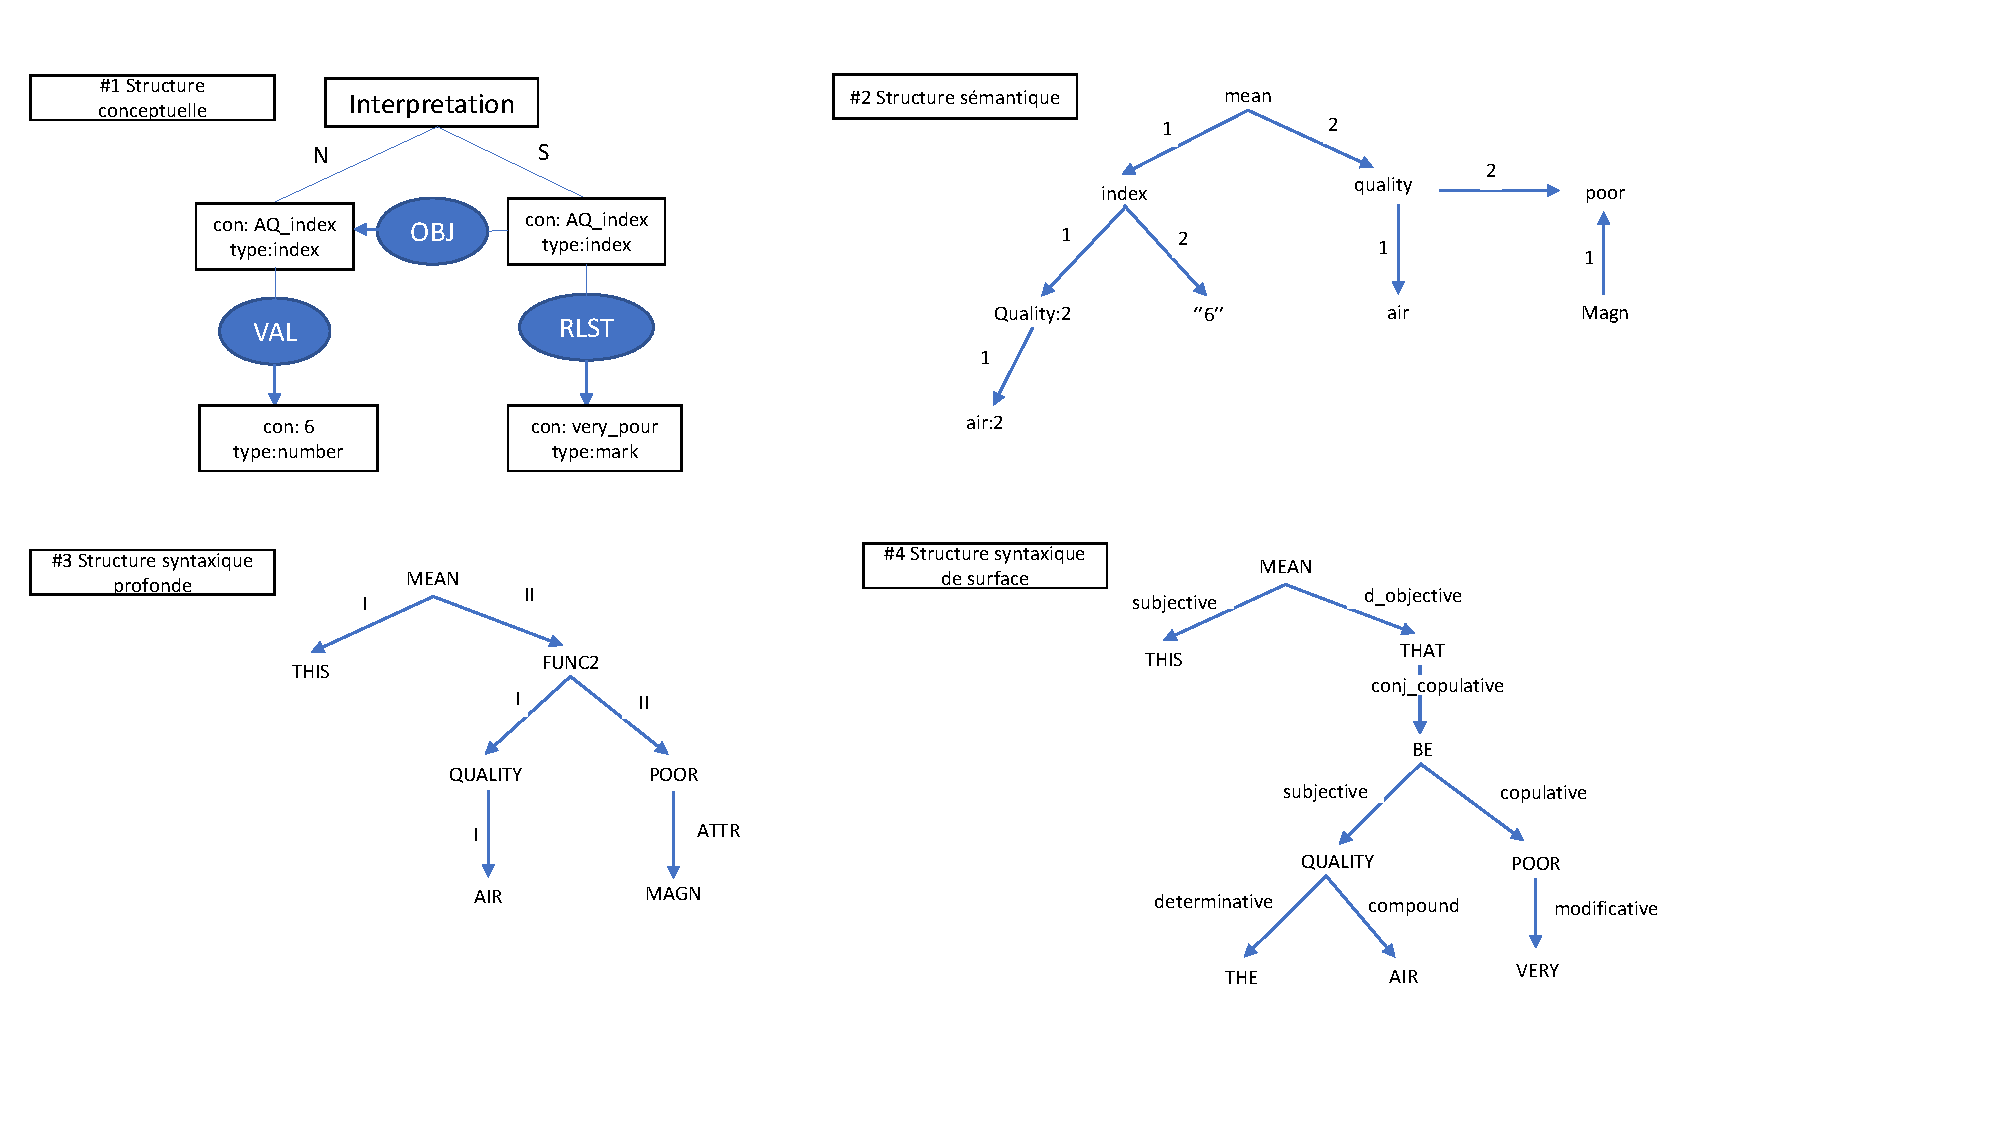
\includegraphics[width=1\textwidth, trim = {0cm 0cm 0cm 0cm},clip]{ch2/figs/marquis.pdf}
	\caption{Pipeline de MARQUIS}
	\label{fig:marquis}
\end{figure}

Puis pour que le transfert d'une interface à l'autre se fasse correctement, MARQUIS a un système de restrictions sur les noeuds des structures en correspondances. Celles-ci sont ensuite matchés aux traits des entrées lexicales encodéesd dans les dictionnaires utilisés.

grammaire: différents modules de règles. Chaque module traite une interface : conceptuelle-sémantique, sémantique-syntaxe, syntaxe profonde-syntaxe de surface, syntsurf-morpho, morpho-texte linéarisé.

Finalement, dans le cadre de ce mémoire, nous utiliserons aussi un système basé sur MARQUIS. Il s'agit de GenDR \citep{lareau18}: un projet en cours de développement dirigé par François Lareau à l’Observatoire de linguistique Sens-Texte. Le chapitre suivant lui décrira en détails ce réalisateur.